% DSD Lab5 report

\documentclass[10pt]{article}
\usepackage{mathtools, amsmath, amsfonts, amssymb}
\usepackage{hyperref, graphicx, wrapfig, geometry}
\usepackage[makeroom]{cancel}

\usepackage[section]{placeins}
\newgeometry{margin=2cm}

\title{ECSE 323 --- Group 47 Lab 5 Enigma Machine}
\author{Jun Young Shin id. 260499663\\ Timothee Flichy id. 260557686}
\date{\today}

\begin{document}
\maketitle
\section{Introduction}
The enigma machine is a cipher machine which encrypts a string of words or numbers so that a 3rd party will not be able to understand the message. This system was extensively used during the world war 1 and 2 by Germany to plan strategic assault to enemy territory. To encrypt the message, the machine used a set of mechanical rotors and electrical circuit. The each rotor can be set by rotating the rotor and ring, and by changing the encryption type. In total, there is 3 independent rotors. In the electrical circuit, there is a circuit called a reflect and stecker which creates another level of encryption by generation a secondary pattern. This complex encryption system is able to create over 158 million million million combinations with 10 pairs of 26 letters. This makes it almost impossible for a human to decrypt the code. To make it even harder and increase the odd, the combination was changed every 24 hours during world war 2. In the course of Digital System Design, we used VHDL to write electronic version of this mechanical system. This report will explain the procedure of creating this device using the Altera board.

\section{Designing of the Enigma machine}
%Before jumping into the VHDL, we first must understand how to implement the mechanical machine to a hardware. In our case the Altera's Cyclone II FPGA model EP2C20F484C7. In figure \ref{fig:enigma_machine_BD} we can see how the hardware will work.\\

%So here is how the enigma machine will work on the FPGA. The user inputs a letter to be encrypted. When the user click a button called a key\_press, the program receives the letter and sends it to the stecker. Stecker meaning plugboard in German, is a simple version of a fixed rotor. It then passes through the first rotor to get the first encryption. The encryption pattern in shown in figure \ref{fig:rotor_encryption}. The encrypted letter will then pass to the second rotor and to the third rotor.\\

%It will then pass to the reflector which does another encryption. The reflector will encrypt the letter to its mirrored. Meaning, if $'A'$ is mirrored with $'Y'$, if any of the letter is passed to the reflector, the mirrored letter will to output it. The encryption of the reflector can be seen in figure \ref{fig:reflector_encryption}.\\

%The reflected letter will then pass back to the third rotor, to the second rotor, and to the first rotor. It finally come back to the stecker which output the encrypted letter.\\

%------------------------------------------------------------------------------------------------------------------------------------------------------------------------------------------------------------------------------------------------------------------------------------------------------------------------------------------------------------------------------------------------------------

The Enigma Machine is a complex cipher machine that requires many components to properly encrypt text. Each input letter is passed through the system twice before being properly encrypted. On figure \ref{fig:enigma_machine_BD} and figure \ref{fig:Enigma_machine_sch}, you see that how the enigma machine will work.\\
\begin{figure}[!htb]
    \centering
    \includegraphics[width=0.7\textwidth]{./enigma_machine_BD.png}
    \caption{Block diagram of the enigma machine.}
    \label{fig:enigma_machine_BD}
\end{figure}
\begin{figure}[!htb]
    \centering
    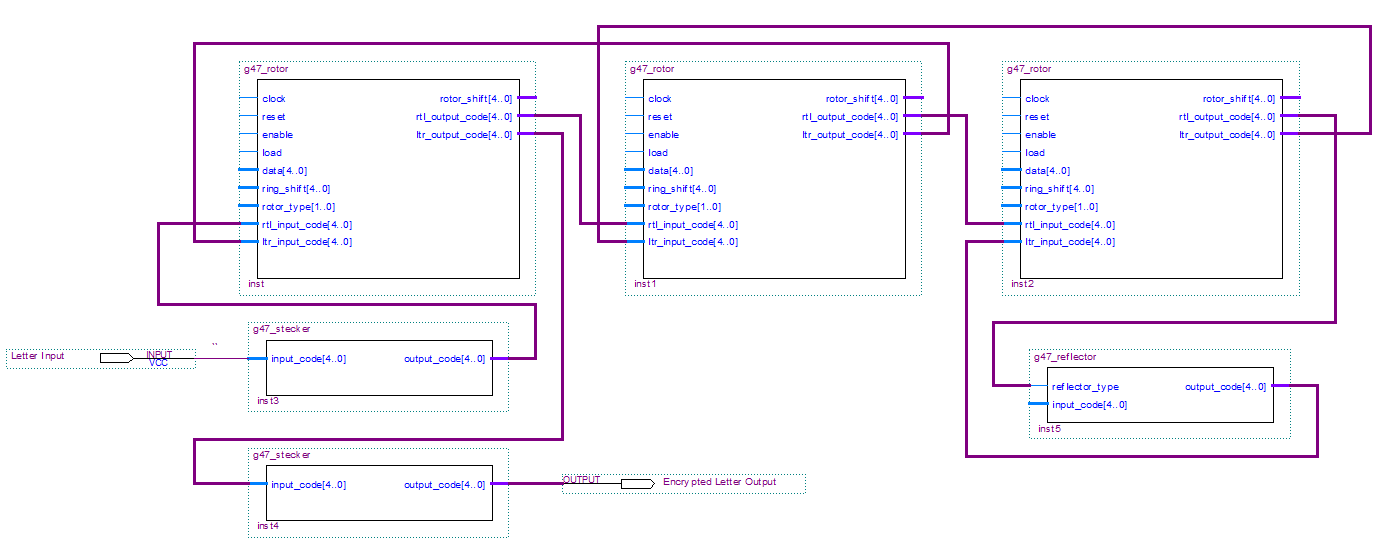
\includegraphics[width=1\textwidth]{./Enigma_machine_sch.png}
    \caption{A simple schematic of the Enigma machine.}
    \label{fig:Enigma_machine_sch}
\end{figure}
\newline
First, the input letter passes through a stecker circuit seen in figure \ref{fig:stecker_layout}, which adds an additional scrambling step by exchanging each letter with precisely one other letter. While the Stecker circuit implemented in the original Enigma machine was a plugboard that could change which letters were connected, our machine simply hardcodes these values.\\
\begin{figure}[!htb]
    \centering
    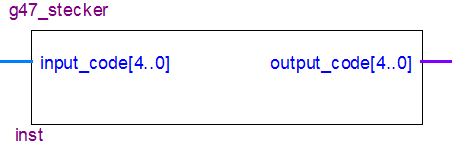
\includegraphics[width=0.3\textwidth]{./stecker_layout.png}
    \caption{The layout of the stecker.}
    \label{fig:stecker_layout}
\end{figure}

Next, the stecker output letter is passed, right to left, through a series of 3 rotors represented in figure \ref{fig:Enigma_machine_sch}. Each rotor has 3 initial settings: the type, the ring setting, and the initial position. Internally, the rotor has an inner core that implements a permutation (based on the rotor type). Depending on the position of the rotor, the rotor input is barrel shifted rightwards before applying that permutation. Additionally, each rotor also has a ring which also shifts the input (leftwards) before the permutation (this happens after the positional shift). After the permutation, the letter is shifted again by the ring and position shift amounts, first by the ring and then by the position (opposite to previous direction). The rotor permutations are shown in figure \ref{fig:rotor_encryption}, corresponding to the rotor type.
\begin{figure}[!htb]
    \centering
    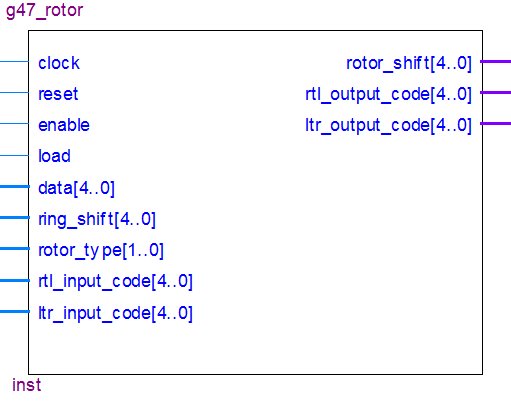
\includegraphics[width=0.3\textwidth]{./rotor_layout.png}
    \caption{The layout of the rotor.}
    \label{fig:rotor_layout}
\end{figure}
\begin{figure}[!htb]
    \centering
    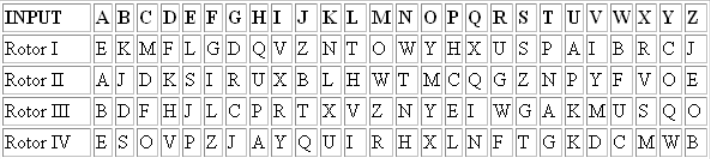
\includegraphics[width=0.6\textwidth]{./rotor_encryption.png}
    \caption{Encryption pattern for the rotor.}
    \label{fig:rotor_encryption}
\end{figure}
\newpage
Finally, the output of the last rotor is passed to a reflector circuit which is shown in figure \ref{fig:reflector_layout}. The reflector has two types, which are hardcoded, and swaps letters similarly to the stecker circuit. The reflector pattern can be seen in figure \ref{fig:reflector_encryption}.
\begin{figure}[!htb]
    \centering
    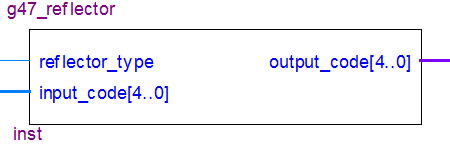
\includegraphics[width=0.5\textwidth]{./reflector_layout.png}
    \caption{The layout of the reflector.}
    \label{fig:reflector_layout}
\end{figure}
\begin{figure}[!htb]
    \centering
    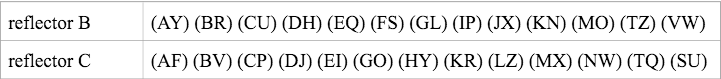
\includegraphics[width=0.5\textwidth]{./reflector_encryption.png}
    \caption{Encryption pattern for the reflector.}
    \label{fig:reflector_encryption}
\end{figure}
The output of the reflector is passed back through the rotors, using the inverse permutation for each rotor, and the stecker circuit. This provides our system with the final encrypted letter.

\section{User Interface}
In order to provide a simple User Interface (UI) to an end user, we decided to use a simple combination components for input and output. You can see the layout of the control on the Altera board on the figure \ref{fig:Altera_ui}.\\
\begin{figure}[!htb]
    \centering
    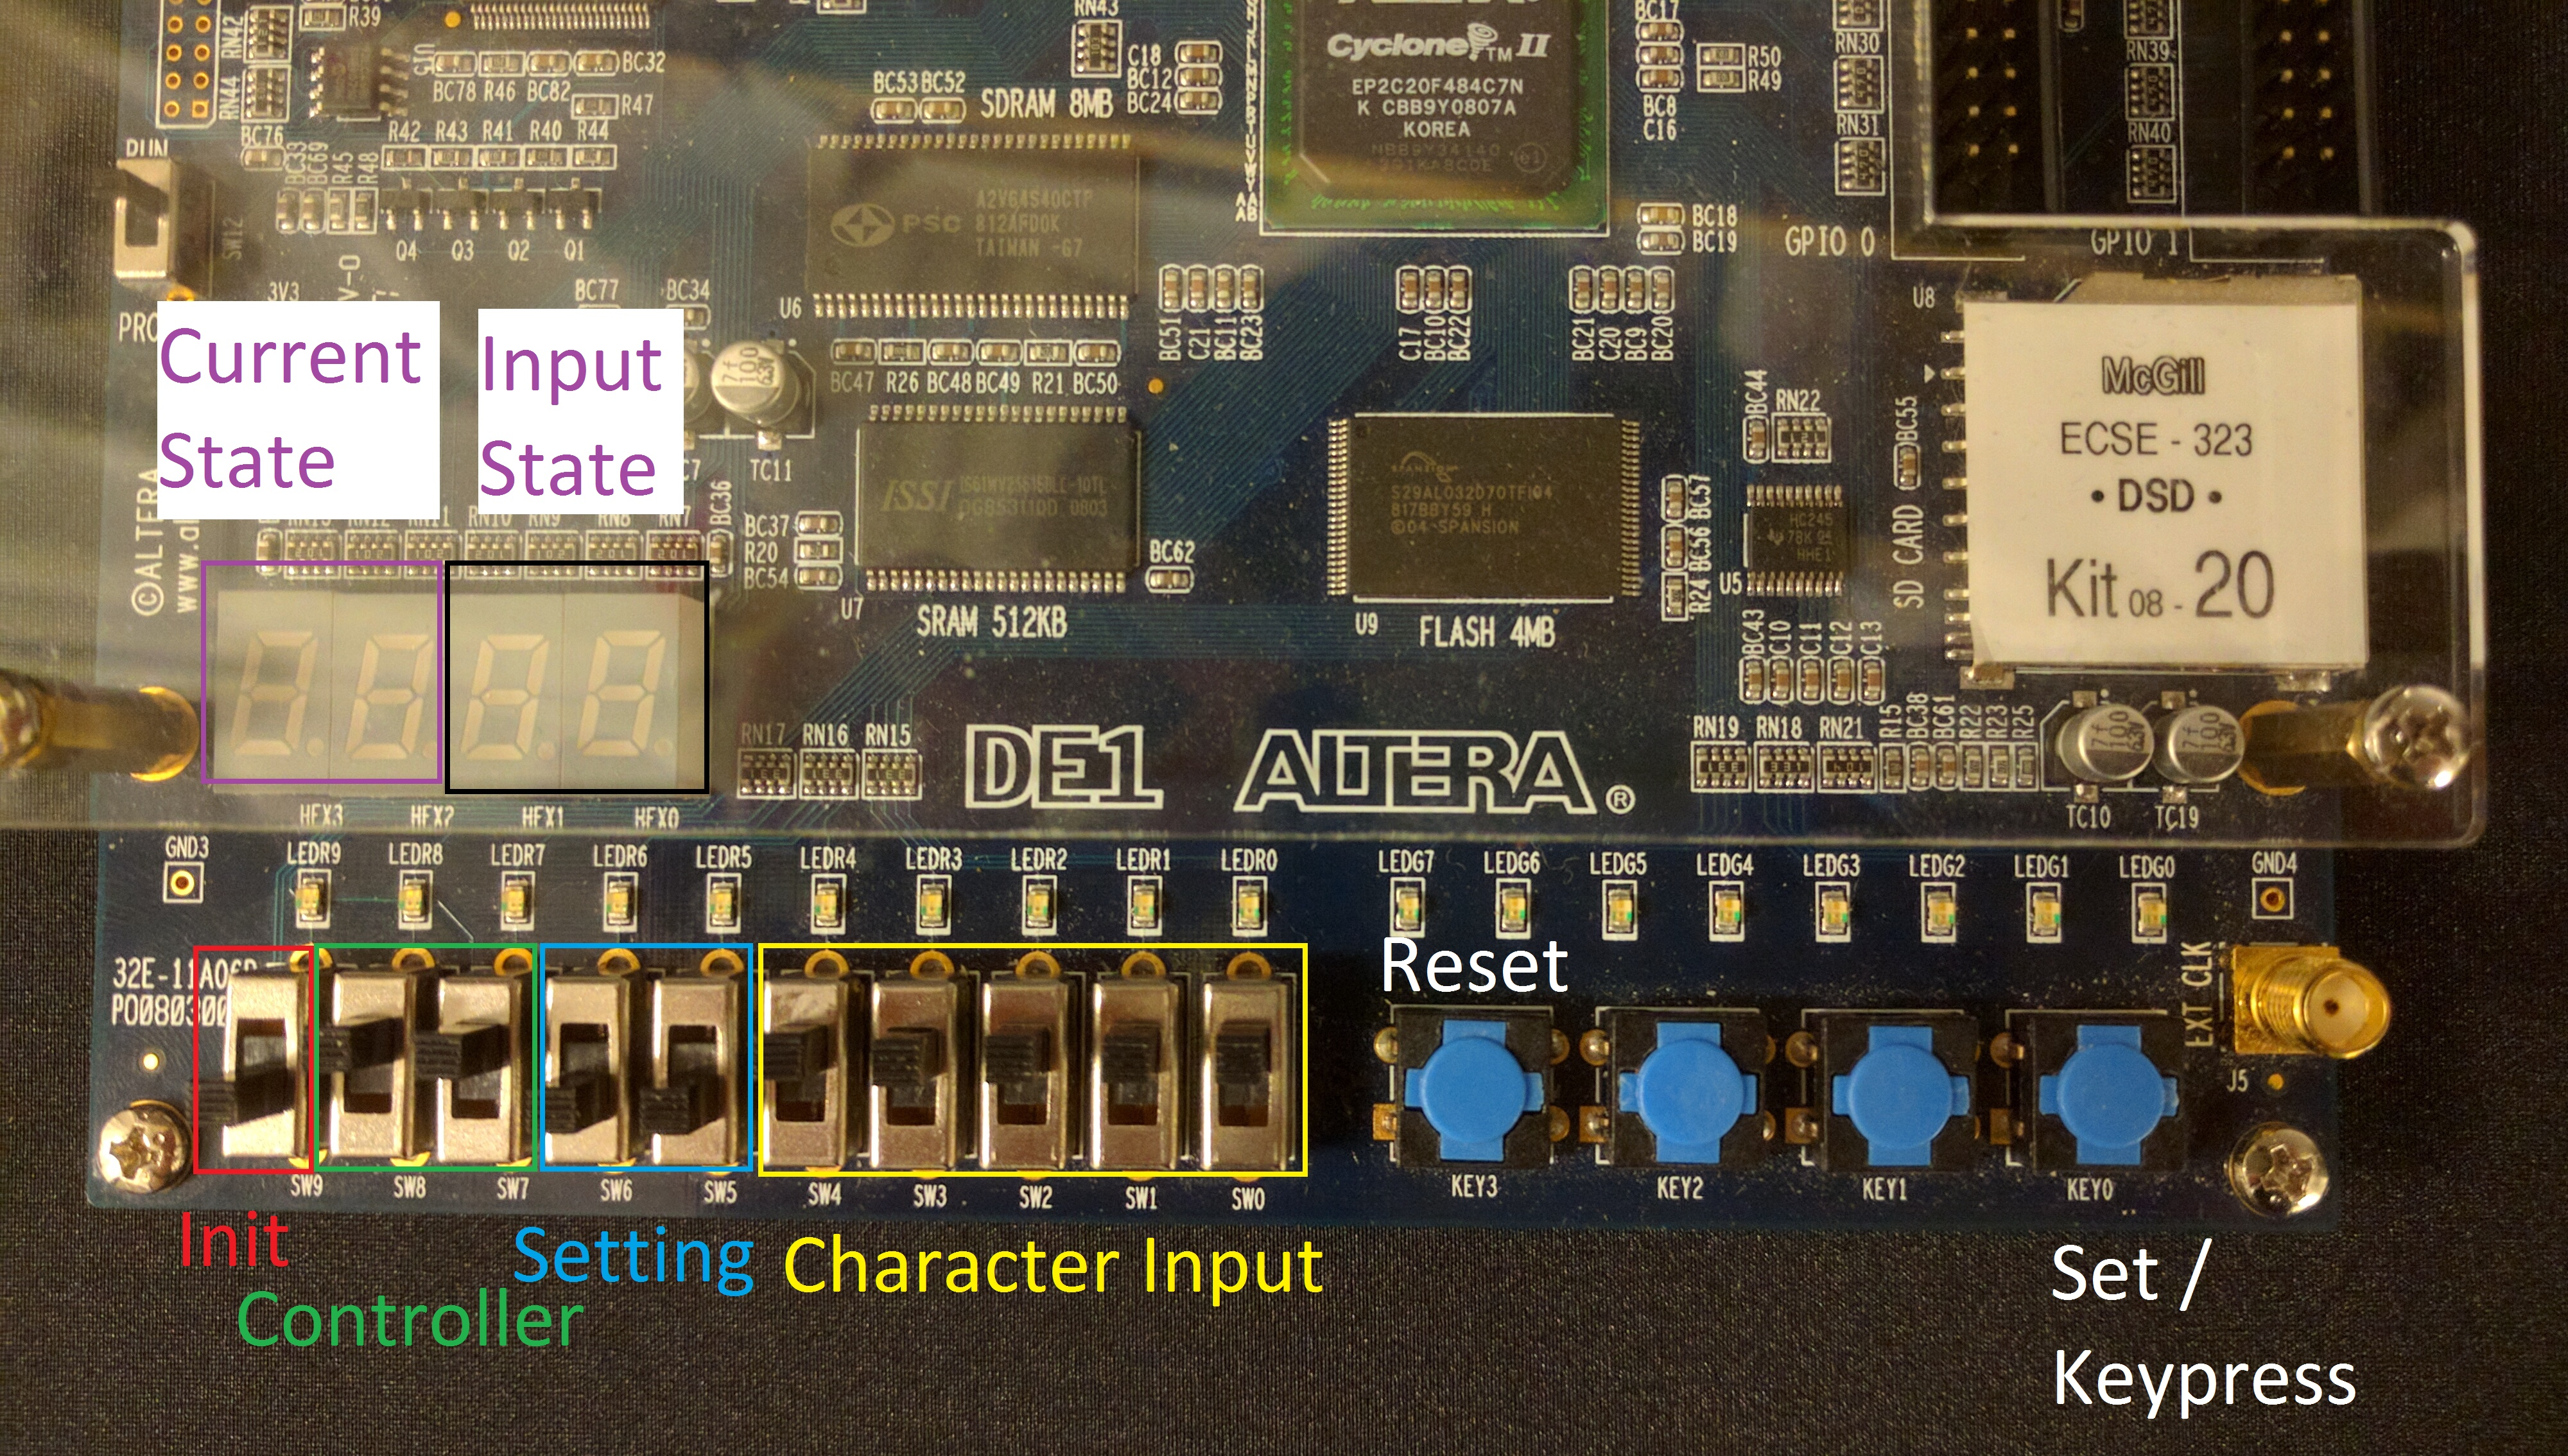
\includegraphics[width=0.7\textwidth]{./Altera_ui.png}
    \caption{User Interface layout on the Altera Board.}
    \label{fig:Altera_ui}
\end{figure}
The UI uses switches as the primary input source, alongside two push-buttons. For the Enigma machine, there are two main modes of operation: initialization and encryption. Therefore, it made sense to assign Switch $SW9$ to control the mode of operation. While initializing the machine we have a total of 10 settings to determine: 3 settings per rotor as well as the reflector type. We decided to use Switches $SW7$ and $SW8$ to control which component we were setting (right, middle, left, or reflector). The setting being changed was determined by Switches $SW5$ and $SW6$, depending on the type of component we were changing. For the Rotors, binary values 0-2 are used for each initial setting. The reflector, on the other hand, ignores the setting type since it only has one setting. The last 5 Switches $SW4$ to $SW0$ are used to indicate input values. In order to simulate a keypress, we use Pushbutton $KEY0$ as a validation button for the current input setting. Lastly, we use Pushbutton $KEY3$ as an asynchronous circuit reset.\\

The UI relies mostly on the hex displays to inform the user what is currently being done. No matter what operation mode we're in, we use Hex 0 and 1 to display the current input value. During initialization, Hex 2 and 3 are used to display the system's current value. During encryption, these displays instead display the encrypted value (after the keypress). Finally, since pushbutton debouncing is tricky, we use the green LED 0-4 to display the number of times the button has been pressed (modulus 26).\\

\section{Testing of the Enigma machine}
In laboratory 5, we had to create a stecker, a reflector, and a rotor. These components are a very important part of the enigma machine, as you can see from the figure \ref{fig:enigma_machine_BD}. After writing the g47\_stecker.vhdl and the g47\_reflector.vhdl, we tested the circuit to make sure it is working as it should. In the figure \ref{fig:stecker_test} we can see the input and the output of stecker. In the figure \ref{fig:refector_0_test} and figure \ref{fig:refector_1_test}.
\begin{figure}[!htb]
    \centering
    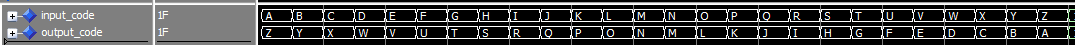
\includegraphics[width=1\textwidth]{./stecker_test.png}
    \caption{The tested output and input of the stecker.}
    \label{fig:stecker_test}
\end{figure}
\begin{figure}[!htb]
    \centering
    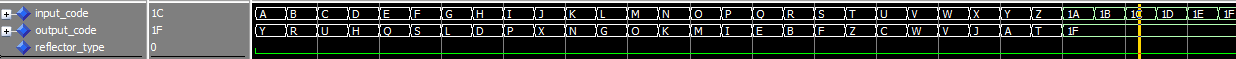
\includegraphics[width=1\textwidth]{./refector_0_test.png}
    \caption{The tested output and input of the reflector at type 0.}
    \label{fig:refector_0_test}
\end{figure}
\begin{figure}[!htb]
    \centering
    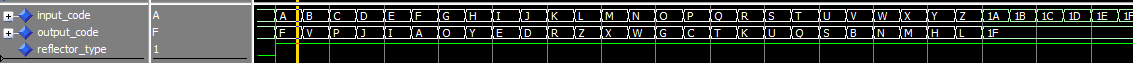
\includegraphics[width=1\textwidth]{./refector_1_test.png}
    \caption{The tested output and input of the reflector at type 1.}
    \label{fig:refector_1_test}
\end{figure}
Knowing that the stecker and reflector function as intended, we completed the design of the enigma machine as seen in figure \ref{fig:Enigma_machine_sch}.\\
In order to test our design, we first performed a functional simulation of our enigma machine. We tested every letter of the alphabet with certain input conditions and made sure that the decrypted output was correct. Additionally, once our UI was completed, we performed several tests by setting specific initial conditions, choosing a message code, and encrypting a small message.
\begin{figure}[!htb]
    \centering
    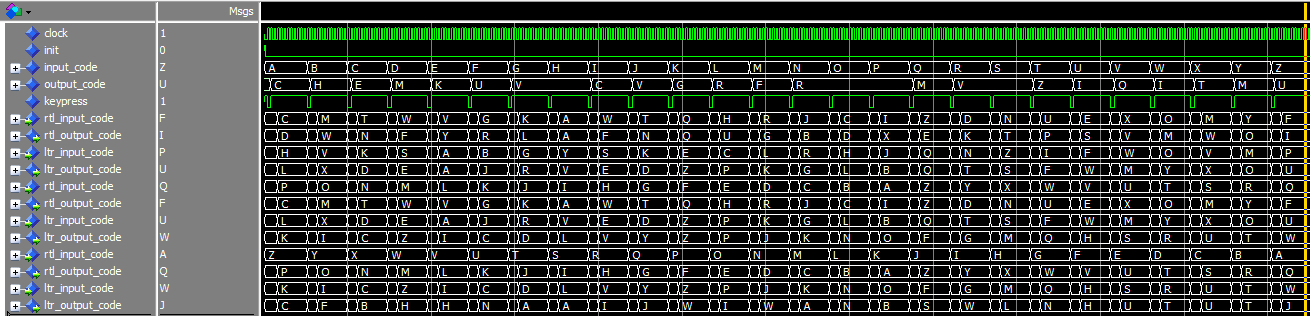
\includegraphics[width=1\textwidth]{./enigma_machine_test.png}
    \caption{The tested output and input of the enigma machine.}
    \label{fig:enigma_machine_test}
\end{figure}
In the figure \ref{fig:enigma_machine_test}, we tested the circuit by setting all the rotor type II, the initial position to be at $'A'$ and the ring setting to be at $'A'$ for each rotor. The reflector was set to type $'0'$. The rest of the rtl\_input\_code, rtl\_output\_code, ltr\_input\_code and ltr\_output\_code are the input and output of each rotor. The pins can be viewed on the figure \ref{fig:rotor_layout}. We can see from the test on figure \ref{fig:enigma_machine_test} that at every key press, the machine accepts the input letter and output the encrypted letter accordingly.\\
For the timing of the enigma machine, we get $"$Fast Model Hold Slack Value$"$ of 0.215, a $"$Slow Model Setup Slack Value$"$ of -1.616 and $"$Slow Model Fmax$"$ of 43.04MHz. The negative slow model setup slack is noticed on the board when testing it as the initiation problem at first. To resolve the issue, we need to set initialization switch to high and then back to low to fix the issue.

\section{Full test on the Altera's FPGA board}
As shown in figure \ref{fig:Altera_ui}, we used all the available switches to be able to set the initial setting of each rotor and the reflector. To test if our UI works perfectly on our system, we test input characters. We will be using the letter $"$A, B, C, D and E$"$ in order. First we set every to $'0'$. The output that we get from the board is $"$K, Y, X, U and N$"$. If we input the value in order, we get $"$A, B, C, D and E$"$ and this can be seen in figure \ref{fig:letter_encrypt} and figure \ref{fig:encrypt_letter}.
\begin{figure}[!htb]
    \centering
    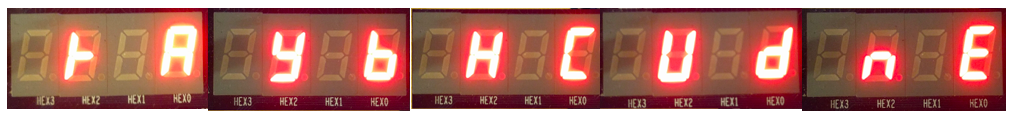
\includegraphics[width=1\textwidth]{./letter_encrypt.png}
    \caption{Input Letter to Encrypted output (Right is the input / left is the output)}
    \label{fig:letter_encrypt}
\end{figure}
\begin{figure}[!htb]
    \centering
    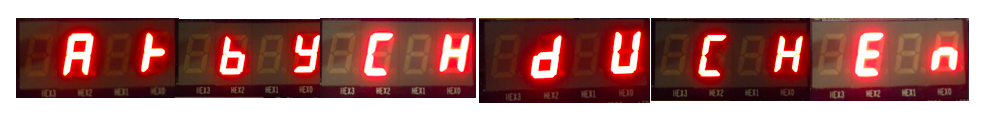
\includegraphics[width=1\textwidth]{./encrypt_letter.png}
    \caption{Encrypted input to Decrypted output (Right is the input / left is the output)}
    \label{fig:encrypt_letter}
\end{figure}
As you can see, the enigma machine works as intended. We also test it by changing the initial conditions. The second test is done by setting reflector to $'1'$ and the middle rotor's ring shifted by 10. With the same input, we get an output of $"$M, P, O, W and X$"$. When the encrypted output in put back to the enigma machine, we get an output of $"$A, B, C, D and E$"$. This concludes that the the UI and enigma machine are both working perfectly.

\section{Conclusion}



\end{document}
